\documentclass{elsarticle}
\usepackage[a4paper,left=2.5cm,right=1.5cm,top=1.5cm,bottom=1.5cm]{geometry}
\usepackage{natbib}
\usepackage{amsmath,amssymb,amsfonts,amsthm}
\usepackage{mathtools}
\usepackage{multirow}
\usepackage[french]{babel}
\usepackage{bm}
\usepackage{algorithmic}
\usepackage{graphicx}
\usepackage{textcomp}
\usepackage{xcolor}
\usepackage{hyperref}
\usepackage{float}
\usepackage[T1]{fontenc}
\usepackage[utf8]{inputenc}
\usepackage{subcaption}
\usepackage{minted}
\graphicspath{{img/}}
\usepackage{svg}
\usepackage{booktabs}
\usepackage{array}
\usepackage{tabularx}
\usepackage{siunitx}
\newcommand{\est}[1]{\multirow{2}{*}{\SI{#1}{\hour}}}
\newcommand{\estbis}[1]{\SI{#1}{\hour}}

\makeatletter
\def\ps@pprintTitle{%
	\let\@oddhead\@empty
	\let\@evenhead\@empty
	\def\@oddfoot{\centerline{\thepage}}%
	\let\@evenfoot\@oddfoot}
\makeatother

\makeatletter
\def\blfootnote{\gdef\@thefnmark{}\@footnotetext}
\makeatother

\def\BibTeX{{\rm B\kern-.05em{\sc i\kern-.025em b}\kern-.08em
		T\kern-.1667em\lower.7ex\hbox{E}\kern-.125emX}}
\usepackage{siunitx}

\newcommand{\abs}{\ensuremath{\textnormal{\inlinedafny|abs|}}}

\newcommand{\ok}{\ensuremath{\textnormal{\inlinedafny|ok|}}}

\DeclareMathOperator{\size}{size}
\DeclareMathOperator{\height}{height}
\DeclareMathOperator{\type}{type}

\renewcommand{\epsilon}{\varepsilon}
\renewcommand{\theta}{\vartheta}
\renewcommand{\kappa}{\varkappa}
\renewcommand{\rho}{\varrho}
\renewcommand{\phi}{\varphi}

\usepackage{textcomp}

\begin{document}
\title{GridFlare --- Optimize Your Signal}
\date{6 mai 2019}

\address[add1]{École Polytechnique, Université catholique de Louvain, Place de l'Université 1, 1348 Ottignies-Louvain-la-Neuve, Belgique}

\author[add1]{Jimmy \textsc{Fraiture}}
\ead{jimmy.fraiture@student.uclouvain.be}

\author[add1]{Edgar \textsc{Gevorgyan}}
\ead{edgar.gevorgyan@student.uclouvain.be}

\author[add1]{Louis \textsc{Navarre}}
\ead{navarre.louis@student.uclouvain.be}

\author[add1]{Gilles \textsc{Peiffer}}
\ead{gilles.peiffer@student.uclouvain.be}

\begin{abstract}
GridFlare est une application Android\texttrademark{} permettant de mesurer la puissance d'un signal Wi-Fi, la latence ou encore les pertes de paquets sur le réseau dans une pièce ou un bâtiment en temps réel ainsi que de sauvegarder les résultats de ces mesures de manière intuitive.
\end{abstract}
\maketitle

\section{Introduction}
L'idée initiale derrière GridFlare était de créer une application mobile sur Android\texttrademark{} permettant de mesurer la puissance de différents signaux dans une pièce, ainsi que d'afficher en continu un résumé des mesures à l'endroit courant.
On pourrait ainsi s'imaginer mesurer la puissance du signal Wi-Fi, d'un signal Bluetooth\textsuperscript{\textregistered}, la qualité du réseau téléphonique, etc..
Ensuite, il serait également possible de sauvegarder ces mesures dans une base de données, en y adjoignant la position, afin d'y avoir accès par la suite.
Grâce à une précision à quelques centimètres, il serait alors possible d'afficher un carte de la pièce, sous forme de heatmap, qui permettrait de visualiser, pour un type de signal donné, la puissance de celui-ci, en interpolant via les points de mesure ajoutés.
Lors de la visualisation, la carte ne concernerait qu'un seul signal, mais il serait possible de changer grâce à une fonctionnalité de \emph{swipe}.

Avec ces fonctionnalités, il serait facile de, par exemple, trouver l'endroit de la pièce voire même du bâtiment entier avec la meilleure puissance de signal afin d'augmenter la productivité chez soi, au travail ou encore dans les endroits ayant un Wi-Fi public.

\begin{figure}[!htbp]
	\centering
	\frame{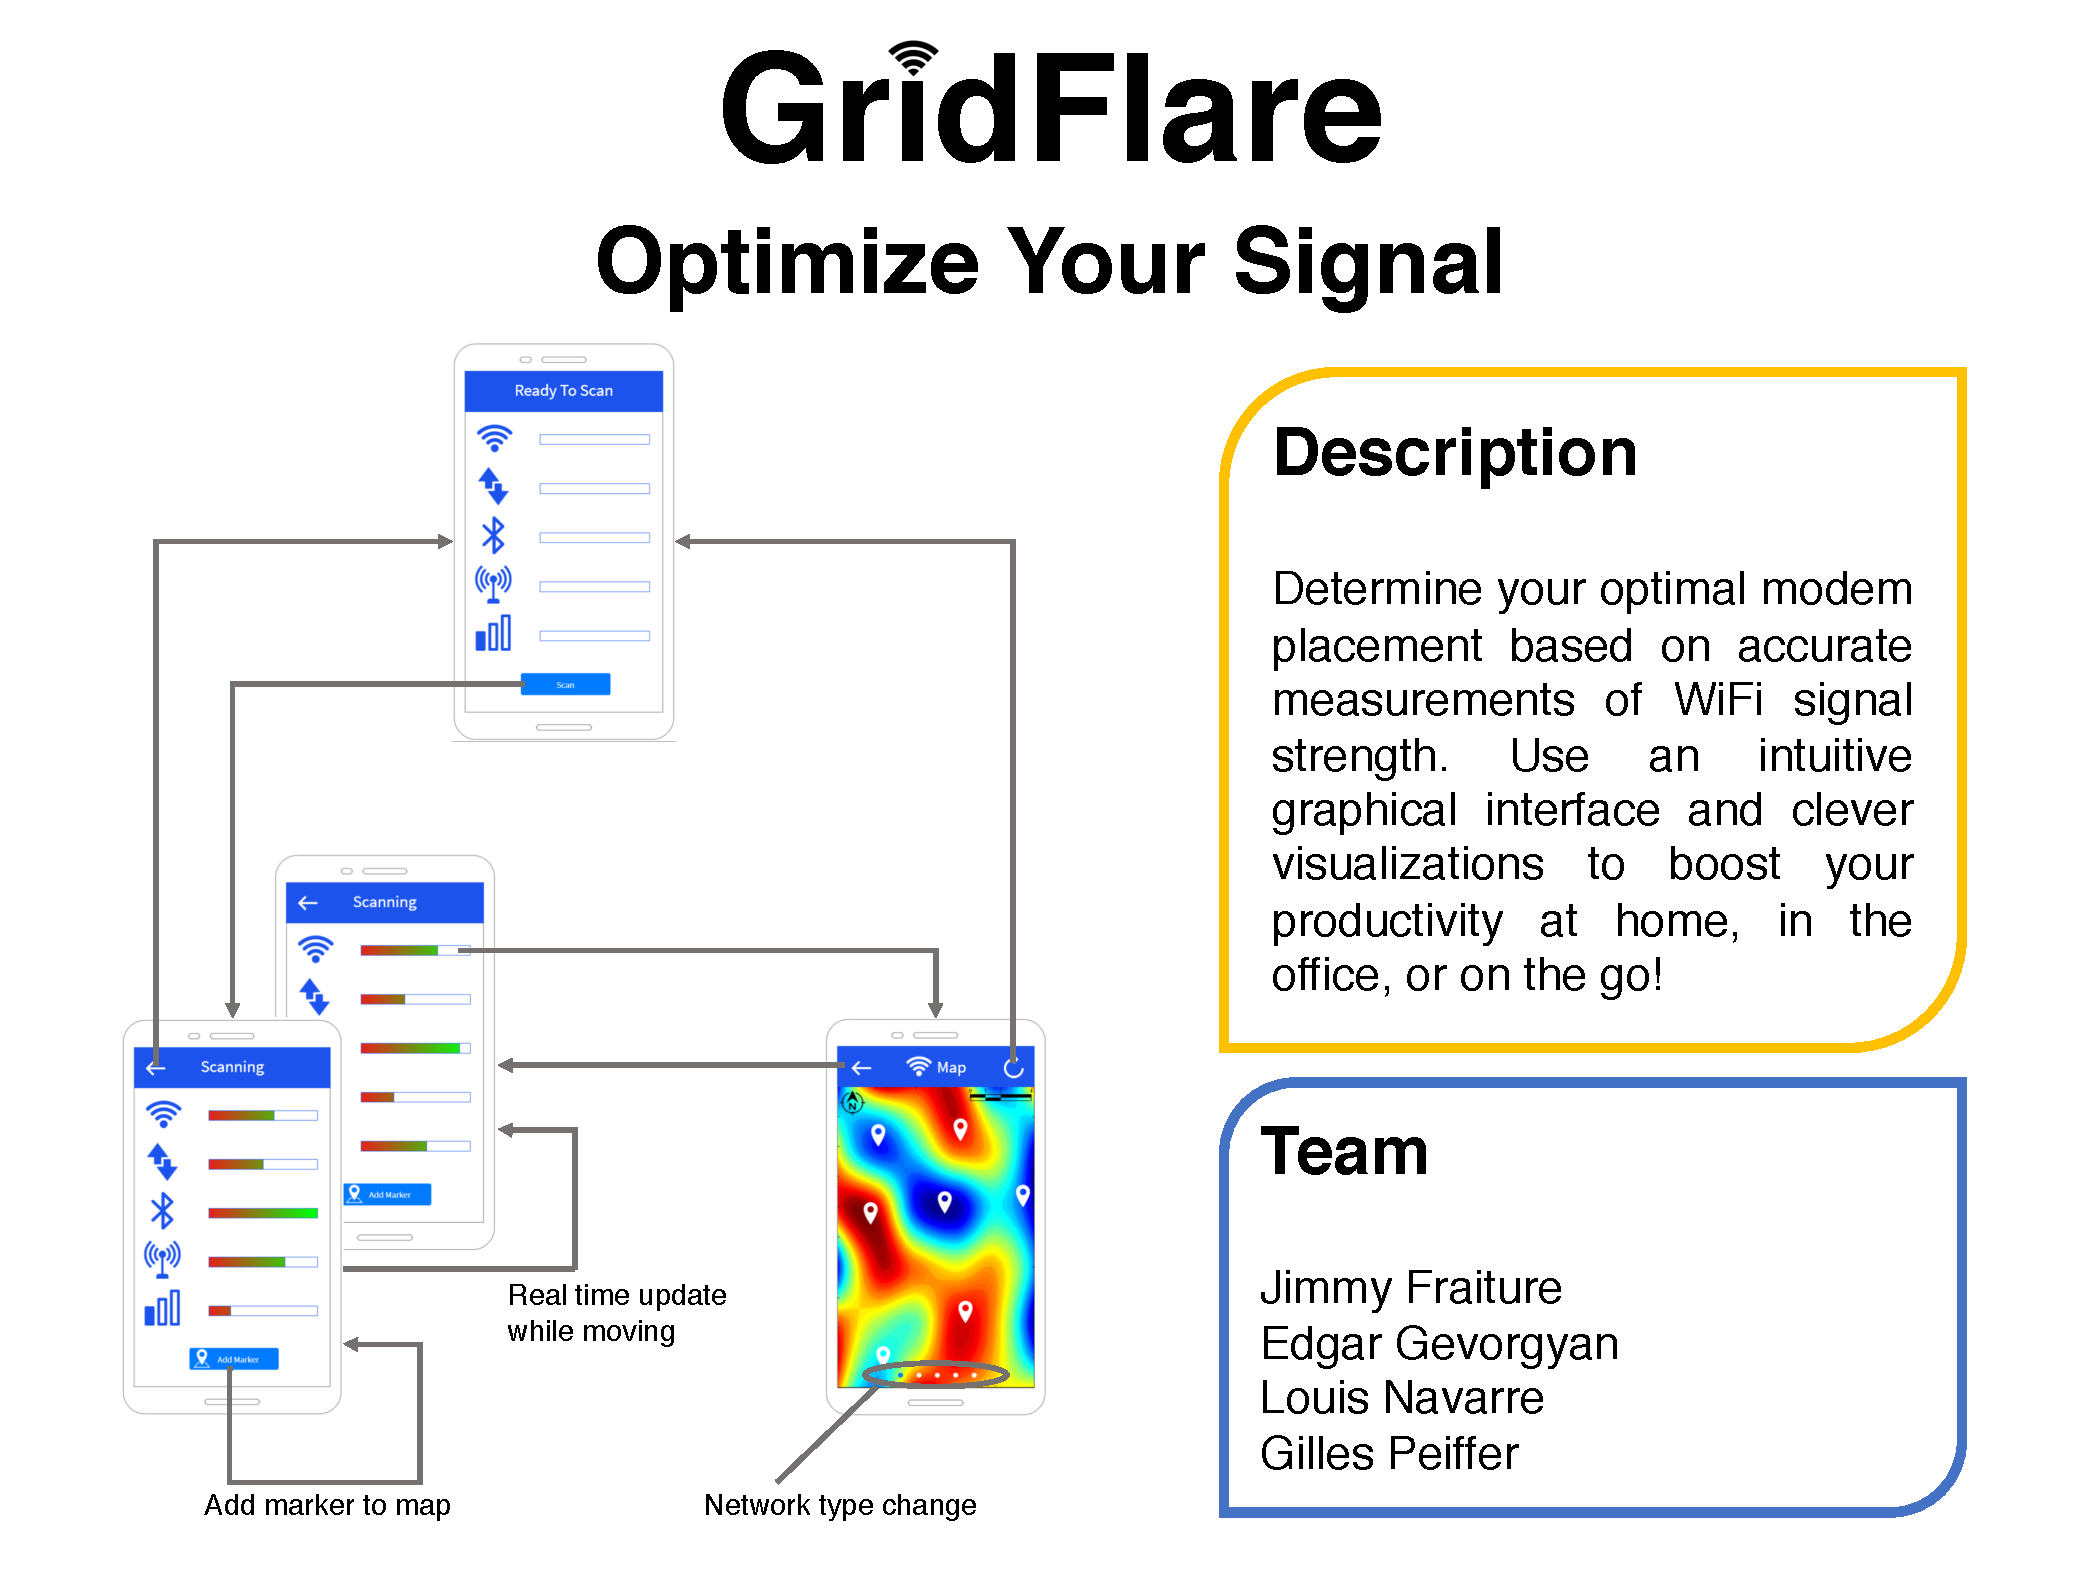
\includegraphics[width=0.8\textwidth]{img/poster_gridflare}}
	\caption{Le poster original de l'application GridFlare, présenté en début de quadrimestre.}
	\label{fig:poster}
\end{figure}

Néanmoins, nous nous sommes rapidement rendus compte que ce ne serait pas possible d'obtenir une résolution suffisamment élevée en ce qui concerne la localisation; en effet, afin de rendre cette application utile, il faudrait au moins avoir accès à une localisation précise à une dizaine de centimètres près, alors qu'avec les outils qui existent actuellement, il est difficile de faire mieux que quelques mètres avec la localisation \textsc{gps}.
D'autres solutions n'étaient également pas envisageables; nous avions pensé à utiliser l'accéléromètre de l'appareil, mais celui-ci est prône aux erreurs, qui en plus s'accumulent rapidement.
Une autre idée serait d'utiliser la caméra de l'appareil, de façon similaire à son utilisation dans, par exemple, les jeux de réalité augmentée.
Cette idée fut également abandonné rapidement en raison de sa complexité démesurée par rapport à la durée du projet.

\section{Rapports de sprint}
\subsection{Premier sprint}
\subsubsection{User stories planifiées}
\begin{table}[H]
	\centering
	\begin{tabular}{p{14cm}m{2cm}}
		\toprule
		\textsc{User story} & \textsc{Estimation}\\
		\midrule
		En tant qu'utilisateur de l'application, je voudrais être capable de mesurer la puissance d'onde de mon Wi-Fi à la position actuelle de mon téléphone. & \est{2}\\
		\midrule
		En tant qu'utilisateur, je souhaite voir des informations supplémentaires par rapport à mon Wi-Fi, comme le ping. & \est{5}\\
		\midrule
		En tant qu'utilisateur, je voudrais pouvoir visualiser la puissance de mon Wi-Fi sur une carte représentant (une partie de) la pièce dans laquelle je me trouve. & \est{30}\\
		\midrule
		En tant qu'utilisateur, je voudrais enregistrer la puissance du Wi-Fi mesuré (à une certaine position). & \est{10}\\
		\midrule
		En tant qu'utilisateur, je souhaite recevoir des informations quant aux endroits où mesurer le Wi-Fi, afin de minimiser le nombre de mesures nécessaires & \est{20}\\
		\bottomrule
	\end{tabular}
\end{table}

\subsubsection{User stories effectuées}
\begin{table}[H]
	\centering
	\begin{tabular}{p{14cm}m{2cm}}
		\toprule
		\textsc{User story} & \textsc{Estimation}\\
		\midrule
		En tant qu'utilisateur de l'application, je voudrais être capable de mesurer la puissance d'onde de mon Wi-Fi à la position actuelle de mon téléphone. & \est{2}\\
		\midrule
		En tant qu'utilisateur, je souhaite voir des informations supplémentaires par rapport à mon Wi-Fi, comme le ping. & \est{8}\\
		\midrule
		En tant qu'utilisateur, je voudrais enregistrer la puissance du Wi-Fi mesuré (à une certaine position). & \est{7}\\
		\bottomrule
	\end{tabular}
\end{table}

\subsubsection{Améliorations pour le prochain sprint}
\begin{itemize}
	\item Continuer notre recherche sur une méthode efficace pour visualiser la puissance de l’onde Wi-Fi sur une carte.
	\item Trouver une façon de calculer le maillage rapidement.
	\item S’intéresser à d’autres types de signaux comme la 3/4/5G.
\end{itemize}

\subsection{Deuxième sprint}
\subsubsection{User stories planifiées}
\begin{table}[H]
	\centering
	\begin{tabular}{p{14cm}m{2cm}}
		\toprule
		\textsc{User story} & \textsc{Estimation}\\
		\midrule
		En tant qu'utilisateur, je souhaite avoir une interface ludique quand j'effectue un test de Wi-Fi. & \est{7}\\
		\midrule
		En tant qu'utilisateur, je souhaite avoir accès à une heatmap me montrant la puissance de mon Wi-Fi au mètre près. & \est{30}\\
		\midrule
		En tant qu'utilisateur, je souhaite avoir accès à un historique des test effectués, en reprenant toutes les informations utiles (date, lieu, ping, \ldots). & \est{5}\\
		\bottomrule
	\end{tabular}
\end{table}

\subsubsection{User stories effectuées}
\begin{table}[H]
	\centering
	\begin{tabular}{p{14cm}m{2cm}}
		\toprule
		\textsc{User story} & \textsc{Estimation}\\
		\midrule
		En tant qu'utilisateur, je souhaite avoir une interface ludique quand j'effectue un test de Wi-Fi. & \est{5}\\
		\midrule
		En tant qu'utilisateur, je souhaite avoir accès à un historique des tests effectués, en reprenant toutes les informations utiles (date, lieu, ping, \ldots). & \est{7}\\
		\bottomrule
	\end{tabular}
\end{table}

\subsubsection{Améliorations pour le prochain sprint}
\begin{itemize}
	\item Les historiques seront faits par pièce (en faisant une moyenne des scans).
	\item Proposer un système de lancement de scan total,
	c’est-à-dire qu’on entre le nombre total de pièces à scanner, faire tous les scans, et obtenir un résumé à la fin.
	\item Trouver un moyen d'avoir une précision au mètre près.
\end{itemize}

\subsection{Troisième sprint}
\subsubsection{User stories planifiées}
\begin{table}[H]
	\centering
	\begin{tabular}{p{14cm}m{2cm}}
		\toprule
		\textsc{User story} & \textsc{Estimation}\\
		\midrule
		En tant qu'utilisateur, je souhaite avoir accès à l'historique par lieu/date de test/pièce, avec la moyenne pour une pièce donnée pour un test effectué à un moment donné. & \est{7}\\
		\midrule
		En tant qu'utilisateur, je souhaite pouvoir lancer un scan complet d'un lieu. & \estbis{5}\\
		\midrule
		En tant qu'utilisateur, je souhaite pouvoir ajouter autant de pièces et de lieux que je souhaite (sans éviter les conflits). & \est{2}\\
		\midrule
		En tant qu'utilisateur, je souhaite pouvoir envoyer par mail un rapport d'un scan complet effectué pour un certain lieu. & \est{8}\\
		\bottomrule
	\end{tabular}
\end{table}

\subsubsection{User stories effectuées}
\begin{table}[H]
	\centering
	\begin{tabular}{p{14cm}m{2cm}}
		\toprule
		\textsc{User story} & \textsc{Estimation}\\
		\midrule
		En tant qu'utilisateur, je souhaite avoir accès à l'historique par lieu/date de test/pièce, avec la moyenne pour une pièce donnée pour un test effectué à un moment donné. & \est{5}\\
		\midrule
		En tant qu'utilisateur, je souhaite pouvoir lancer un scan complet d'un lieu. & \estbis{15}\\
		\midrule
		En tant qu'utilisateur, je souhaite pouvoir ajouter autant de pièces et de lieux que je souhaite (sans éviter les conflits). & \est{3}\\
		\midrule
		En tant qu'utilisateur, je souhaite pouvoir envoyer par mail un rapport d'un scan complet effectué pour un certain lieu. & \est{4}\\
		\bottomrule
	\end{tabular}
\end{table}

\subsubsection{Améliorations pour le prochain sprint}
\begin{itemize}
	\item Améliorer le côté visuel (pour l'instant il faut presque mettre Eiffel 65 en collaborateurs\ldots).
	\item Réarranger la manière dont les activités s’enchaînent.
	Pour l’instant, trois activités se ressemblent mais font des choses différentes.
	On s’y perd un peu; il faut clean tout ça.
	Par exemple tout ce qui concerne les lieux (ajouter, supprimer, consulter l'historique, commencer un nouveau scan) dans la même activité.
\end{itemize}

\subsection{Quatrième sprint}
\subsubsection{User stories planifiées}
\begin{table}[H]
	\centering
	\begin{tabular}{p{14cm}m{2cm}}
		\toprule
		\textsc{User story} & \textsc{Estimation}\\
		\midrule
		En tant qu'utilisateur, je souhaite pouvoir distinguer et inférer clairement le but des différents menus de l'application grâce à une interface intuitive. & \est{25}\\
		\midrule
		En tant qu'utilisateur, je souhaite pouvoir effacer automatiquement les scans pour une pièce/un lieu donné(e) lorsque j'efface cette pièce/ce lieu. & \est{2}\\
		\midrule
		En tant qu'utilisateur, je souhaite pouvoir modifier un lieu ou une pièce après l'avoir créé(e), en mettant à jour les scans existants. & \est{5}\\
		\bottomrule
	\end{tabular}
\end{table}

\subsubsection{User stories effectuées}
\begin{table}[H]
	\centering
	\begin{tabular}{p{14cm}m{2cm}}
		\toprule
		\textsc{User story} & \textsc{Estimation}\\
		\midrule
		En tant qu'utilisateur, je souhaite pouvoir distinguer et inférer clairement le but des différents menus de l'application grâce à une interface intuitive. & \est{30}\\
		\midrule
		En tant qu'utilisateur, je souhaite pouvoir effacer automatiquement les scans pour une pièce/un lieu donné(e) lorsque j'efface cette pièce/ce lieu. & \est{5}\\
		\midrule
		En tant qu'utilisateur, je souhaite pouvoir modifier un lieu ou une pièce après l'avoir créé(e), en mettant à jour les scans existants. & \est{4}\\
		\bottomrule
	\end{tabular}
\end{table}


\subsubsection{Améliorations pour le prochain sprint}
\begin{itemize}
	\item Continuer de déplacer les fonctionnalités présentes dans l'ancien UI vers la nouvelle interface.
	\item Améliorer le bot email.
	\item Détecter et enlever les bugs restants dans l'application (clavier qui ne disparaît pas, \ldots).
	\item Rendre l'utilisation plus fluide et claire.
	\item Passer aux \mintinline{java}{ViewPager}s pour améliorer la vitesse de transition des \mintinline{java}{Fragment}s.
	\item Stocker et utiliser la date des scans.
	\item Permettre la création de pièces dans les scans ponctuels.
\end{itemize}

\subsection{Cinquième sprint}
\subsubsection{User stories planifiées}
\begin{table}[H]
\centering
\begin{tabular}{p{14cm}m{2cm}}
	\toprule
	\textsc{User story} & \textsc{Estimation}\\
	\midrule
	En tant qu'utilisateur, je souhaite pouvoir sauvegarder la date d'un scan afin de savoir si mes données sont encore à jour. & \est{2}\\
	\midrule
	En tant qu'utilisateur, je souhaite pouvoir créer des nouvelles pièces lors d'un scan ponctuel. & \est{5}\\
	\midrule
	En tant qu'utilisateur, je souhaite avoir une application qui s'adapte à la taille de mon téléphone, de sorte à pouvoir continuer son utilisation après un changement d'appareil. & \est{10}\\
	\bottomrule
\end{tabular}
\end{table}

\subsubsection{User stories effectuées}
\begin{table}[H]
\centering
\begin{tabular}{p{14cm}m{2cm}}
	\toprule
	\textsc{User story} & \textsc{Estimation}\\
	\midrule
	En tant qu'utilisateur, je souhaite pouvoir sauvegarder la date d'un scan afin de savoir si mes données sont encore à jour. & \est{1}\\
	\midrule
	En tant qu'utilisateur, je souhaite pouvoir créer des nouvelles pièces lors d'un scan ponctuel. & \est{7}\\
	\midrule
	En tant qu'utilisateur, je souhaite avoir une application qui s'adapte à la taille de mon téléphone, de sorte à pouvoir continuer son utilisation après un changement d'appareil. & \est{15}\\
	\bottomrule
\end{tabular}
\end{table}

\section{Manuel d'utilisation}
\section{Conclusion}

\section*{Références}

\bibliography{gridflare-ref}
\bibliographystyle{elsarticle-harv}\biboptions{authoryear}

\end{document}
\endinput